This section describes the development phase of our project. The development was started around the end of the needfinding phase once the team had a clear vision on the problems we were about to address and the solutions to get over those.

\subsection{Proposal}
% what do we propose? 

% what are the scenarios in which the solution can work? 

\subsection{Project planning and tooling}
Right before jumping into the development, the roles of the team members were chosen, the available resources were considered and our availability was analyzed. We discussed how individuals can contribute to the final outcome of the project, how we can use our tutors' resources, what the main milestones in the project are and how much time can the team members dedicate to this project. 

The Gantt chart on Figure \ref{gantt-chart} summarizes the project's timeline, with the main milestones and activities. The purple lines mark the scheduled time for the activity, while the orange lines mark the time frame in which an activity was executed, but not originally planned.
 
\begin{figure}[h] 
		\begin{center}
			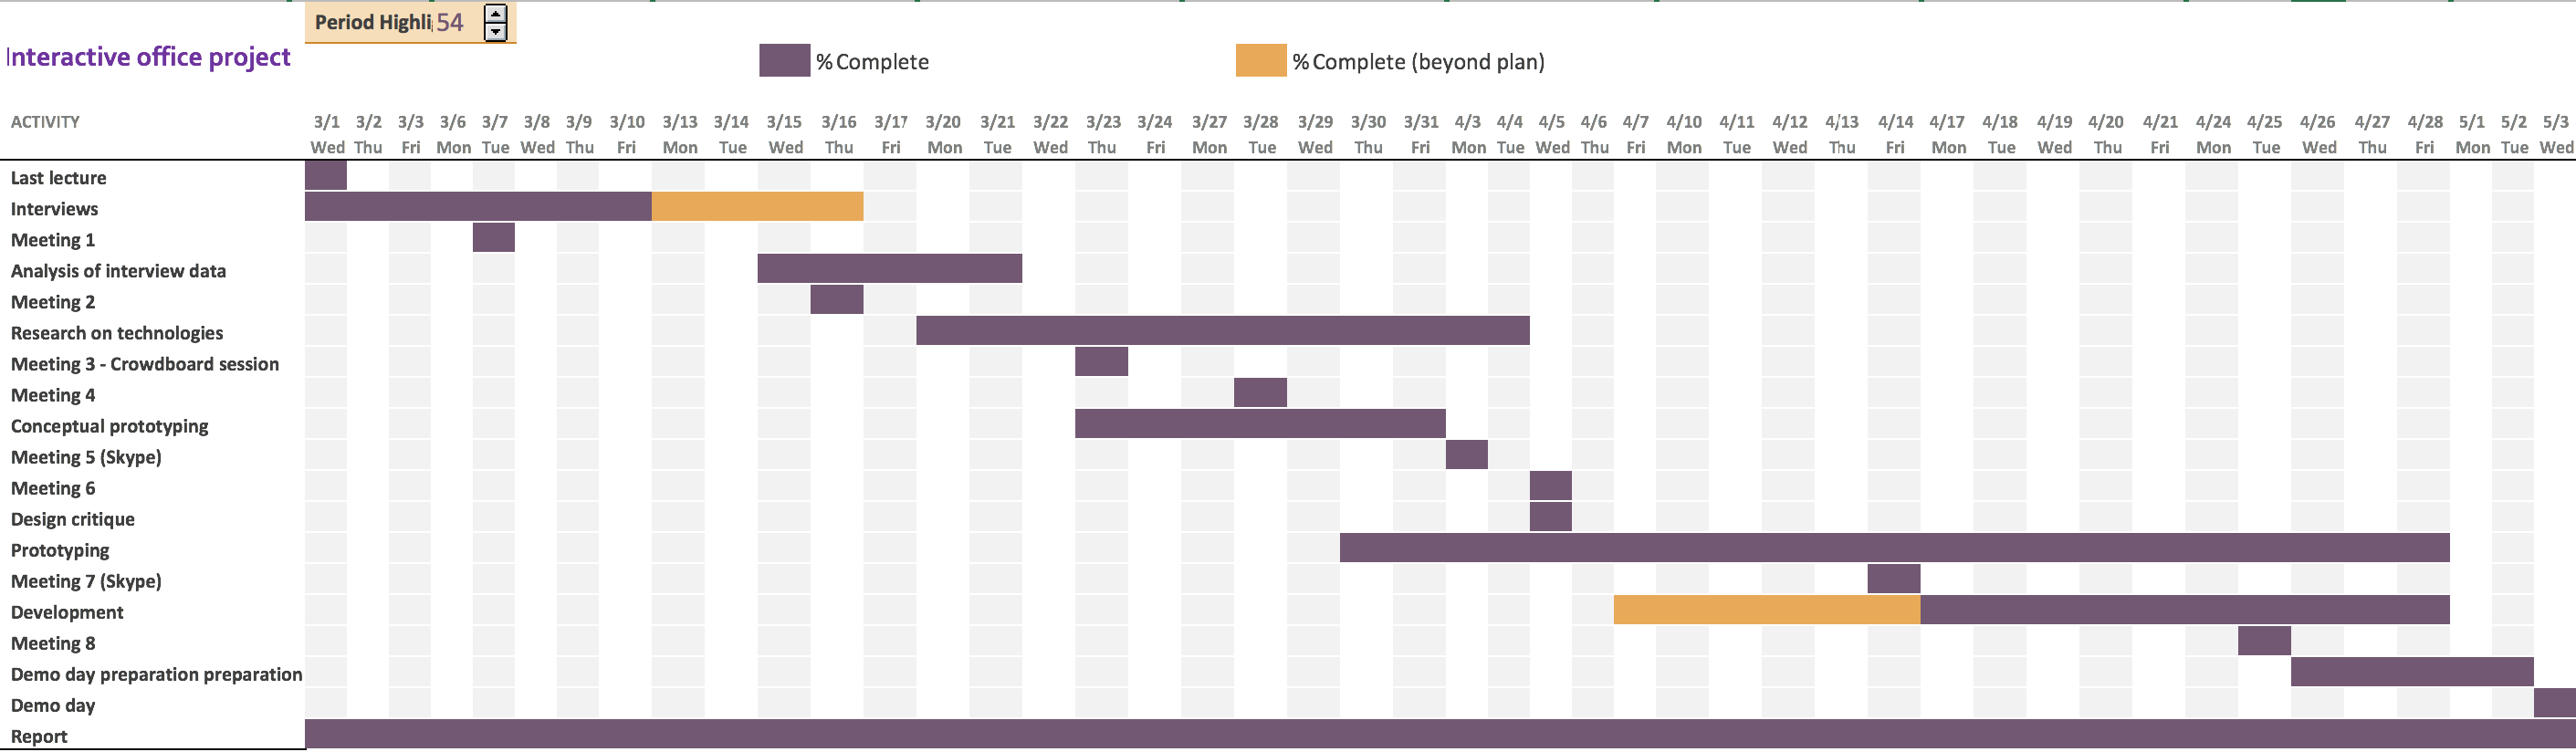
\includegraphics[width=1\textwidth]{images/gantt-chart.png}
			\caption{The Gantt chart of the project.}
			\label{gantt-chart}
		\end{center}
	\end{figure} 
 
% github as a working tool
To make the communication and knowledge sharing among team members, a Facebook group and a Google Drive folder was configured. For future source code version tracking, a Github page\footnote{\url{https://github.com/orgs/InteractiveOfficeProject/}} was configured. The full source code of the project and the report is made available through this page for the public. 

For the wireframes and prototype design, Microsoft Visio was used. To design the APIs, a Swagger \footnote{\url{http://swagger.io}} page was modified. Xamarin IDE \footnote{\url{https://www.xamarin.com/}} (Integrated Developer Environment) was used for the client's development.

\subsection{Chosen technologies}
The application is separated into a client and a server application.
% what resources are utilized for carrying the project out? 

% what technologies, development principles are chosen and followed and why? 

%what do we build upon?

\paragraph{Client} It was decided to develop the client in GTK\#. We chose this framework because it is platform-independent -- our client will be able to run on Linux, MacOS, and Windows -- and we were familiar with C\#. We decided to create a minimum viable product (MVP) and extend this application in small steps. 

A screenshot of the MVP is displayed in Figure \ref{fig:mvp-screenshot}. It has only 2 functionalities: to notify the user the user 25 minutes after work has been started and to notify the user 5 minutes after a break has been started. Both ``starting work'' and ``starting break'' have to be manually triggered by the users via clicking the corresponding buttons.\todo{add next feature extensions}\todo{what resources are utilized for carrying the project out?}\todo{what technologies, development principles are chosen and followed and why? }

\begin{figure}
  \centering
  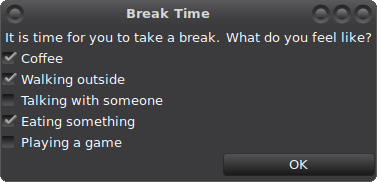
\includegraphics{images/mvp-screenshot.png}
  \caption{Client MVP}
  \label{fig:mvp-screenshot}
\end{figure}



\subsection{APIs}
% what technologies were chosen and why?

